\section{Finite Element Modeling}

When performing optimization to find designs, numerous designs must be analyzed and evaluated for fitness. In some cases, these designs and their fitness functions can be modeled using closed form equations. In the many cases, however, the designs are complex enough that finding closed form models of their behavior is infeasible. In the case that no closed form solutions can be found, numerical analysis can offer an alternative method of evaluating for fitness. 

For this study, numerical analysis in the form of Finite Element Modeling was chosen as the method for evaluating the designs for fitness. Each design and load case each are represented as slight modifications to a basic model file containing the fixed geometry and ``starting" parameters for the design and loading variables.  \todo{Do I need to summarize the basics of finite element modeling?}

This study makes exclusive use of quadrilateral shell elements, known to NASTRAN as \codeword{CQUAD4} elements. These elements are 2-dimensional, but do model deformation in all three dimensions. It should be noted that \codeword{CQUAD4} elements are plate bending elements, relying on the plate equations for their formulations \todo{cite here}. These equations rely on the piece being modeled have a relatively small thickness in relation to their width and depth \cite{reddy}. In the case of the beam flanges, this convention is not followed. Therefore, there will be a loss in accuracy for the stress returned in this region. This is acceptable, as this design is being analyzed to demonstrate the methods outlined here only. The beam flanges are modeled in this inaccurate manner in order to allow flange width to be varied by simply changing the thickness property of the flange material. In a production simulation, another method must be employed to vary the flange thickness.  

\subsection{Selected Model}
\label{sec:model}

\begin{figure}
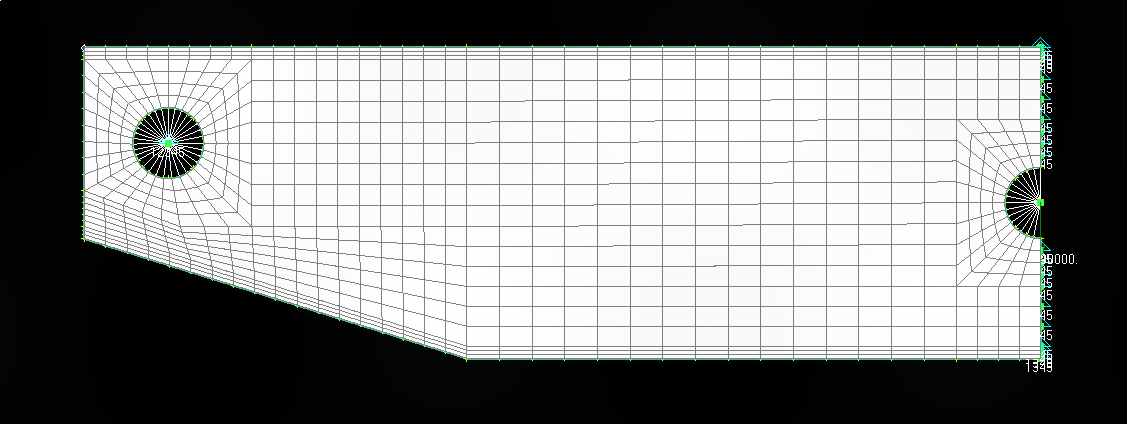
\includegraphics[width=\textwidth]{img/mesh_geom.png}
\caption{Mesh Geometry}
\label{img:mesh_geom}
\end{figure}

The model developed for the example problem considered in this work is shown in figure \ref{img:mesh_geom}. This model was developed using the dimensional data shown in figure \ref{img:dim_beam}. As shown, the model consists of several regions, all of which are modeled using \codeword{CQUAD4} elements. The regions that are of importance for this study are: 

\begin{enumerate}
  \item The top flange
  \item The bottom flange
  \item The web
  \item A thickened region surrounding the hoist mounting lug
  \item A thickened region surrounding the load mounting lug. 
\end{enumerate}

\begin{figure}
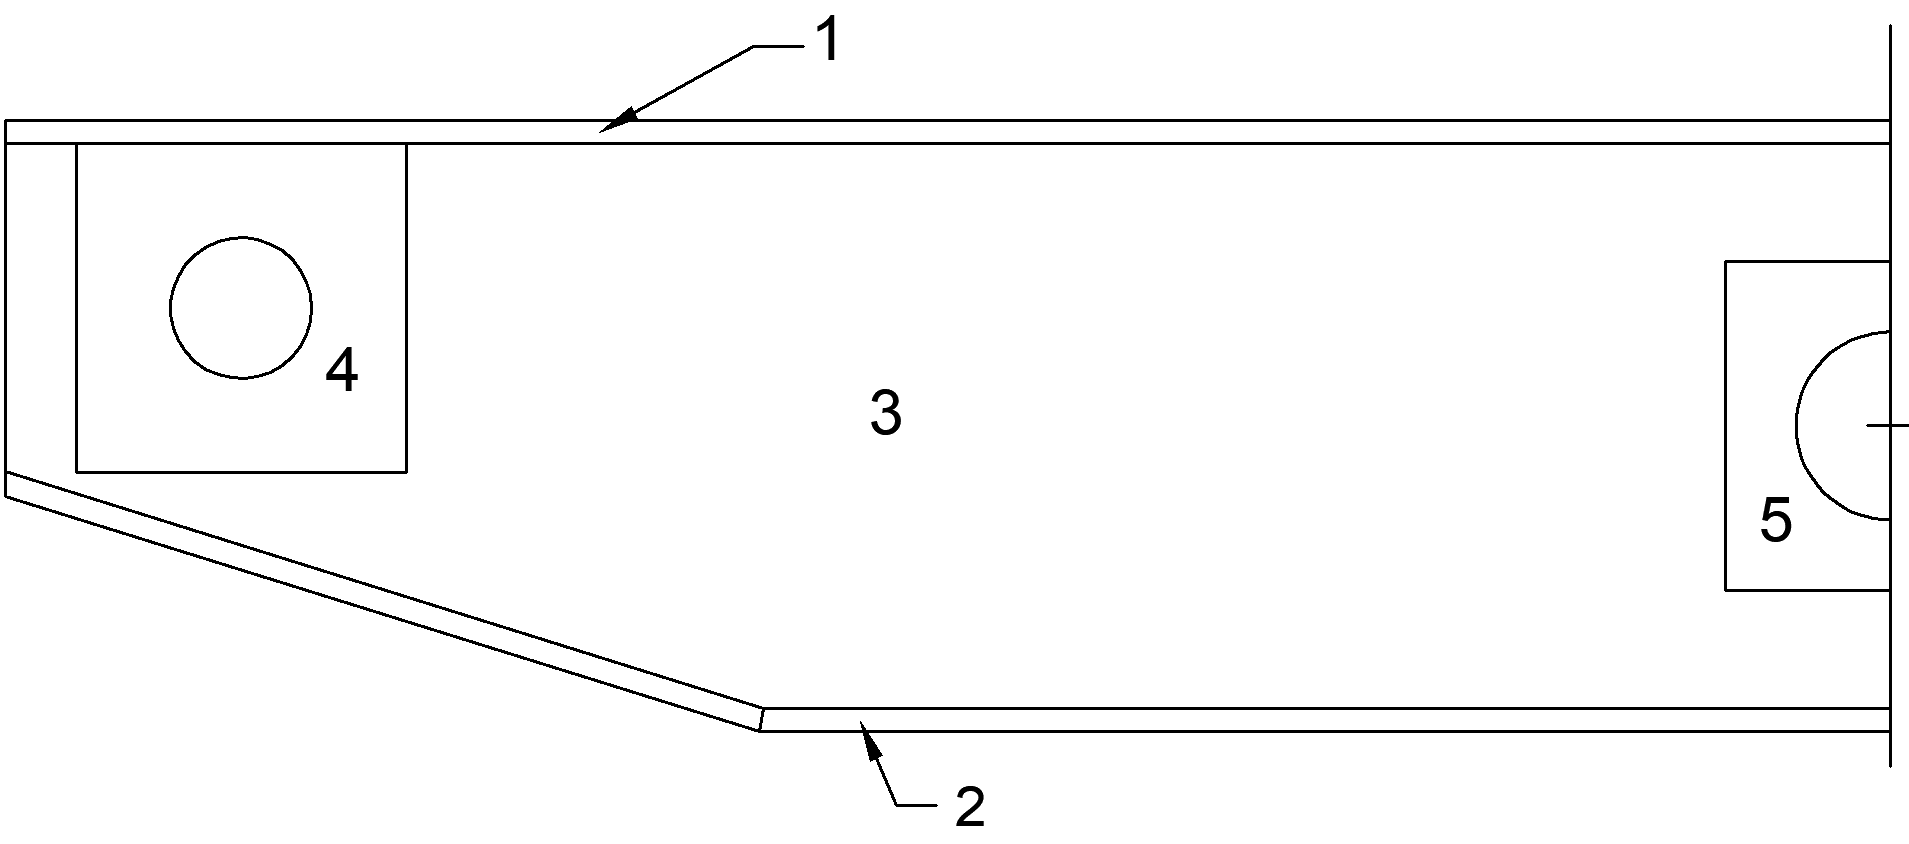
\includegraphics[width=\textwidth]{img/numbered_geom.png}
\caption[Diagram of Modeled Beam]{Diagram of Modeled Beam Showing Region Numbers, Force Locations and Constraints.}
\label{img:num_geom}
\end{figure}

Figure \ref{img:num_geom} shows the named regions as they correspond to portions of the model/drawing. 

Also worth noting is that this model is a partial representation of the whole beam. As the example beam in figure \ref{img:basic_beam} shows, the beam features symmetry along the front view. Due to the typical construction of these beams, they also exhibit symmetry along the top view as well. Because of this, the model presented is only one quarter of the complete beam. To account for this, constraints are imposed along the symmetry cut that simulate the remainder of the beam. 

